\documentclass[12pt]{article}
\usepackage[margin=1in]{geometry}
\usepackage{graphicx}
\usepackage{multicol}

\title{Earl Grey Chocolate Pie}
\author{}
\date{}

\begin{document}

\maketitle

\begin{multicols}{2}
    \section*{Ingredients}
    \subsection*{For the Filling}
    \begin{itemize}
        \item 2 cups + a few splashes of heavy cream
        \item 2 tbsp Earl Grey tea leaves
        \item 2 tbsp sugar
        \item 5 egg yolks
        \item 2 tbsp cornstarch
        \item 7 oz white chocolate
    \end{itemize}

    \subsection*{For the Ganache}
    \begin{itemize}
        \item 1/4 cup + 2 tbsp heavy cream
        \item 3 1/2 oz bittersweet chocolate
    \end{itemize}

    \subsection*{Additional}
    \begin{itemize}
        \item 1 pre-made pie crust
    \end{itemize}

    \columnbreak

    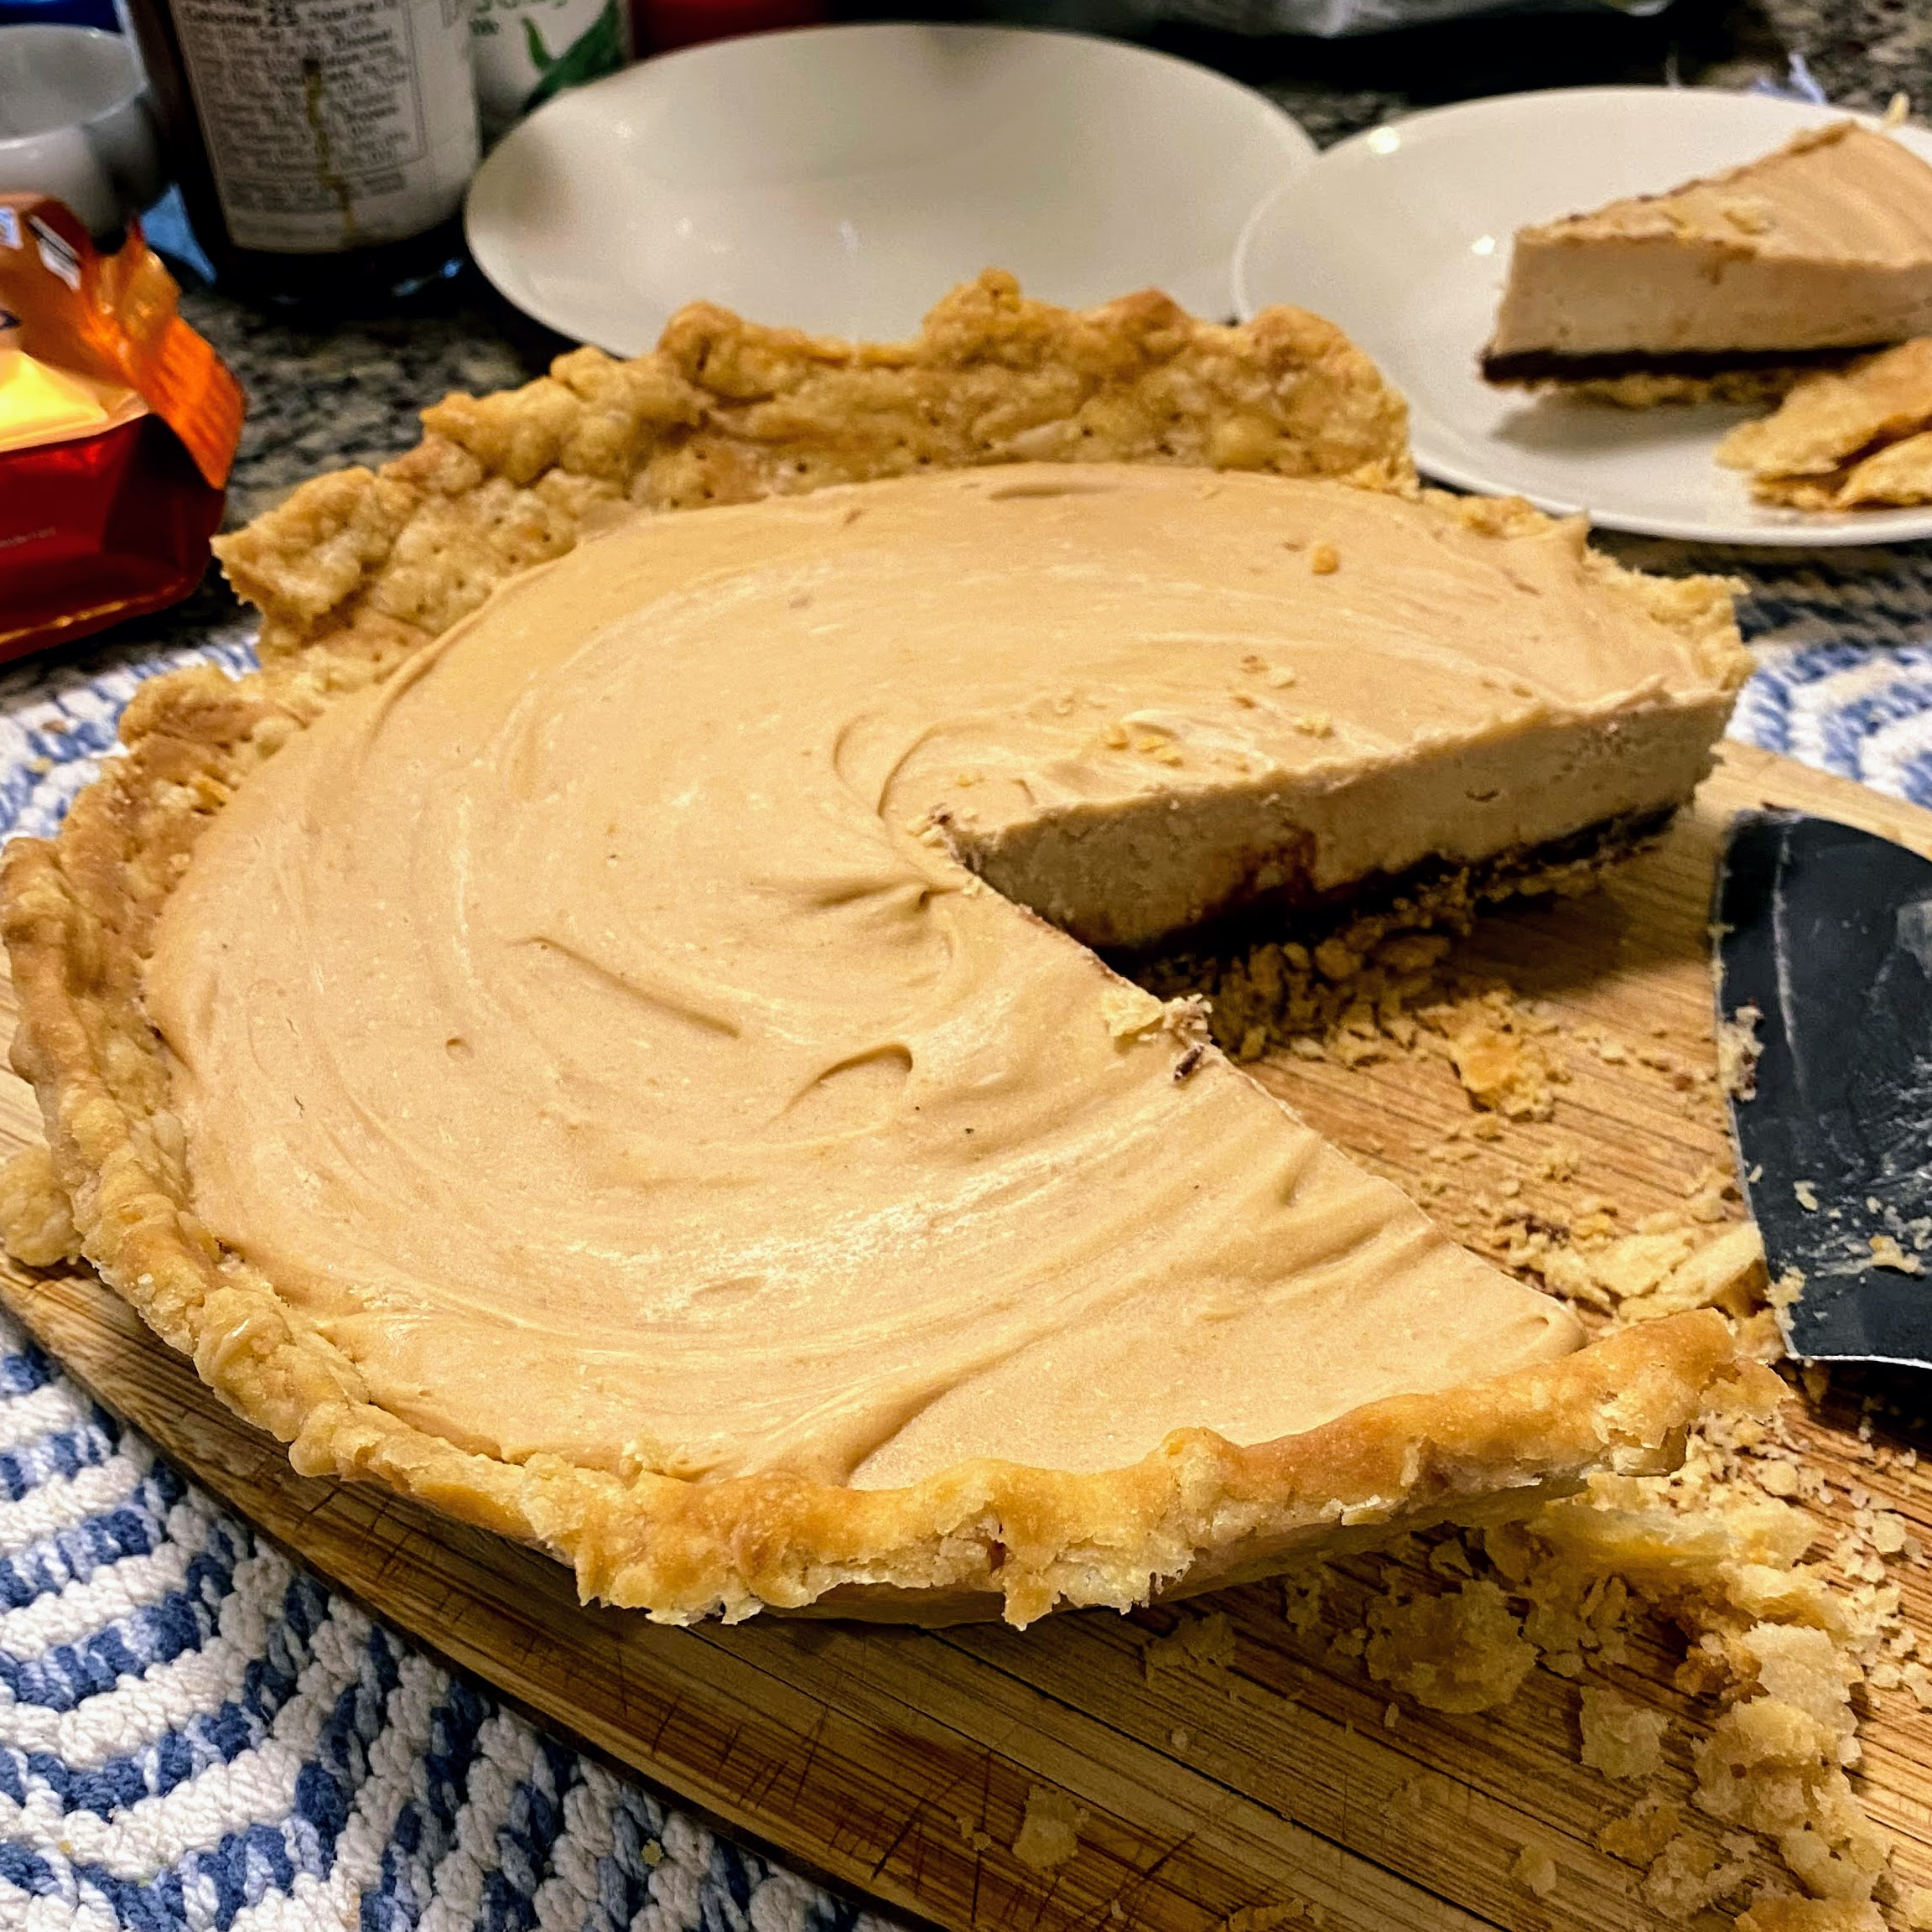
\includegraphics[width=\linewidth]{assets/earl_gray_pie.jpg}
    \centering
    \textit{The Earl Grey Pie}
\end{multicols}

\newpage

\section*{Instructions}
\begin{enumerate}
    \item Have the pie crust ready.
    \item Mix 2 cups of heavy cream with 2 tbsp loose Earl Grey tea in a small pot. Heat until simmering. Let it simmer for 5 minutes, avoiding boiling.
    \item Move the cream to a heat-safe container and put it in the fridge.
    \item Heat 1/4 cup + 2 tbsp heavy cream. Pour over 3 1/2 oz bittersweet chocolate. Stir until the chocolate melts. Heat more in the microwave if needed. Spread on the bottom of the pie crust.
    \item Pour 1 cup of the tea-infused cream into a large bowl, straining out the tea leaves as you do. Put the remainder back in the fridge.
    \item Prepare a double boiler with a large bowl. Add 1 cup of the tea-infused cream and 2 tbsp sugar. Start warming it over the boiler.
    \item In a smaller bowl, whisk 5 egg yolks with 2 tbsp cornstarch.
    \item Slowly add a few spoonfuls of the warm tea-infused cream to the egg mixture while whisking constantly to temper the eggs. This step is crucial to avoid curdling.
    \item Gradually pour the tempered egg mixture back into the double boiler with the rest of the warm cream. Stir constantly while heating until the mixture thickens. Be patient and avoid overheating to prevent curdling.
    \item Once the mixture has thickened, stir in 7 oz of white chocolate until completely melted and smooth. Move the mixture to the fridge to chill.
    \item After 1 hour (or however long it takes for the mixture to cool completely), remove the mixture and the remainder of the tea-infused cream from the fridge. Ensure the mixture is cold.
    \item Strain the remaining tea-infused cream, discarding any tea leaves. Measure to ensure it equals 1 cup; add more cream if necessary.
    \item Whip the cream until peaks form. Carefully fold it into the chilled custard mixture until combined.
    \item Pour the mixture into the prepared pie crust and chill until fully set.
\end{enumerate}

\end{document}
